%!TEX root = ./intern_report.tex

\newpage
\subsection{Py2WFG: A better way to write Wave Flow Graph}
\subsubsection{Python Vs. WFG}

\begin{figure}[h]
    \centering
    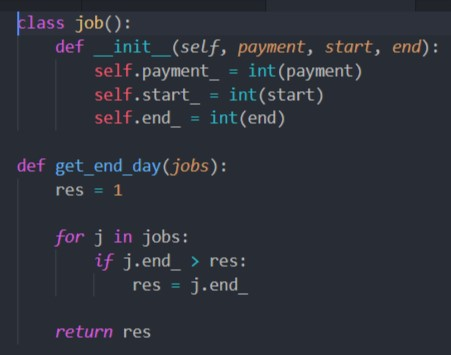
\includegraphics[trim=0cm 0cm 0cm 0cm, clip=true,scale=0.5]{figures/py_eg.jpg}
    \caption{Typical Python code snippet\label{Fig:pyeg}}\vspace{-4mm}
    \end{figure}

\paragraph{}
The Figure~\ref{Fig:pyeg} shows a typical python code example and Figure~\ref{Fig:wfgstruct} shows a WFG snippet. These two languages were built for two entirely different purposes but the highly adaptable nature of python makes a valid point whether if it can replace the functionality of WFG. But both languages have their pros and cons.

\subsubsection*{Python}
\paragraph{}
Python is a general purpose scripting language which focuses on user friendliness. It supports object oriented programming and is also backed up by a huge number of highly optimized libraries for various purposes. But when compared with languages such as C++ and Java, Python is heavy on the memory and slow for large volume computing. It is also not optimized for the particular purpose of programming the Wave DPU.

\subsubsection*{WFG}
\paragraph{}
WFG was created with one purpose and one purpose only in mind, Programming the Wave DPU. Thus it has primary operators that can precisely match the deep capabilities of the DPU hardware. It can be very efficient too when properly programmed. The downside to this language is that it is very strongly typed and is a user friendliness nightmare. Repetitive operators need to be manually entered by the user and the language has no capability of any kind of looping of the language itself.

\subsubsection{Enter Py2WFG}
\paragraph{}
A solution was created by taking the best of both worlds
 